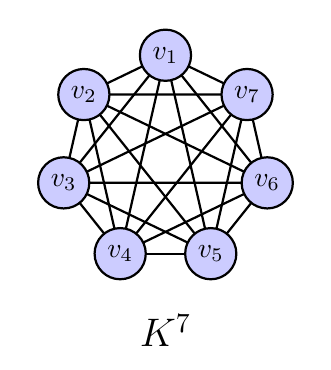
\begin{tikzpicture}[
  baseline=0pt,
  scale=0.7,
  vnode/.style={circle, draw=black, fill=blue!20, thick, inner sep=0pt, minimum size=6.5mm},
  edge/.style={thick, draw=black}
]
  \useasboundingbox (-2.5,-3.4) rectangle (2.5,2.3);

  \begin{scope}[yshift=-0.094cm]
    % Coordenadas con ángulos exactos
    \foreach \i in {1,...,7} {
      \pgfmathsetmacro{\ang}{90 + (\i-1)*360/7}
      \coordinate (v\i) at (\ang:1.894);
    }

    % Aristas
    \foreach \i in {1,...,6} {
      \pgfmathtruncatemacro{\start}{\i+1}
      \foreach \j in {\start,...,7} {
        \draw[edge] (v\i) -- (v\j);
      }
    }

    % Vértices
    \foreach \i in {1,...,7} {
      \node[vnode] at (v\i) {$v_\i$};
    }
  \end{scope}

  % Etiqueta
  \node[font=\Large] at (0,-3.2) {$K^7$};
\end{tikzpicture}
